\documentclass{article}
\usepackage[margin=0.5in]{geometry}
\usepackage[utf8]{inputenc}
\usepackage{textcomp}

\usepackage{pgfplots}
\pgfplotsset{width=10cm,compat=1.9}
%\usepgfplotslibrary{external}
%\tikzexternalize

\begin{document}
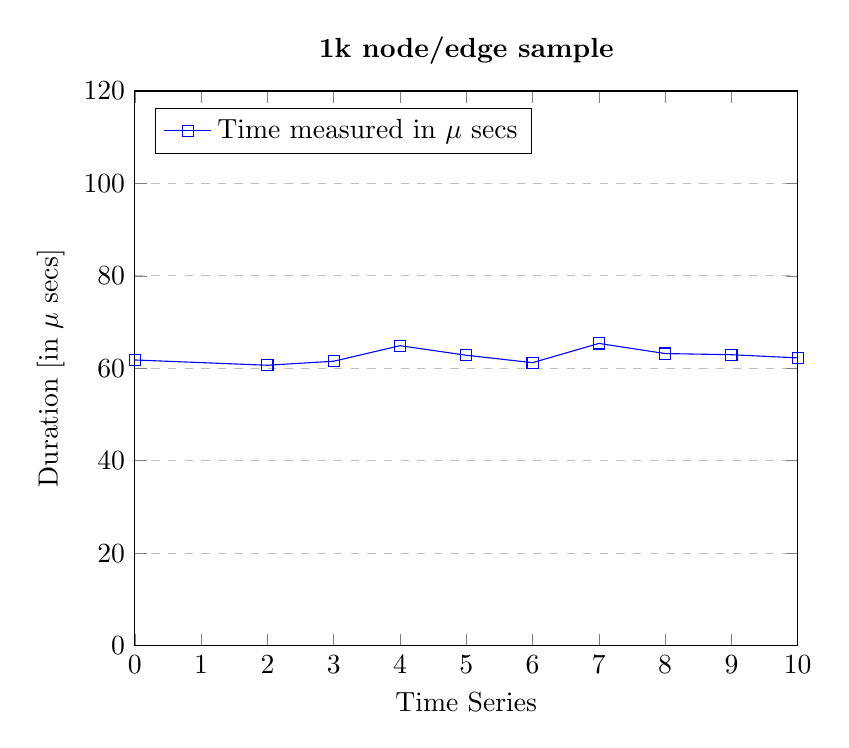
\begin{tikzpicture}

\begin{axis}[
    title=\textbf{1k node/edge sample},
    xlabel={Time Series},
    ylabel={Duration [in $\mu$ secs]},
    xmin=0, xmax=10,
    ymin=0, ymax=120,
    xtick={0,1,2,3,4,5,6,7,8,9,10},
    ytick={0,20,40,60,80,100,120},
    legend pos=north west,
    ymajorgrids=true,
    grid style=dashed,
]

\addplot[
    color=blue,
    mark=square,
    ]
    coordinates {
    (0,61.79)(2,60.65)(3,61.52)(4,64.88)(5,62.81)(6,61.21)(7,65.37)(8,63.18)(9,62.93)(10,62.24)
    };
    \legend{Time measured in $\mu$ secs}
    
\end{axis}
\end{tikzpicture}\newline\newline


%==================SEPARATOR========================%


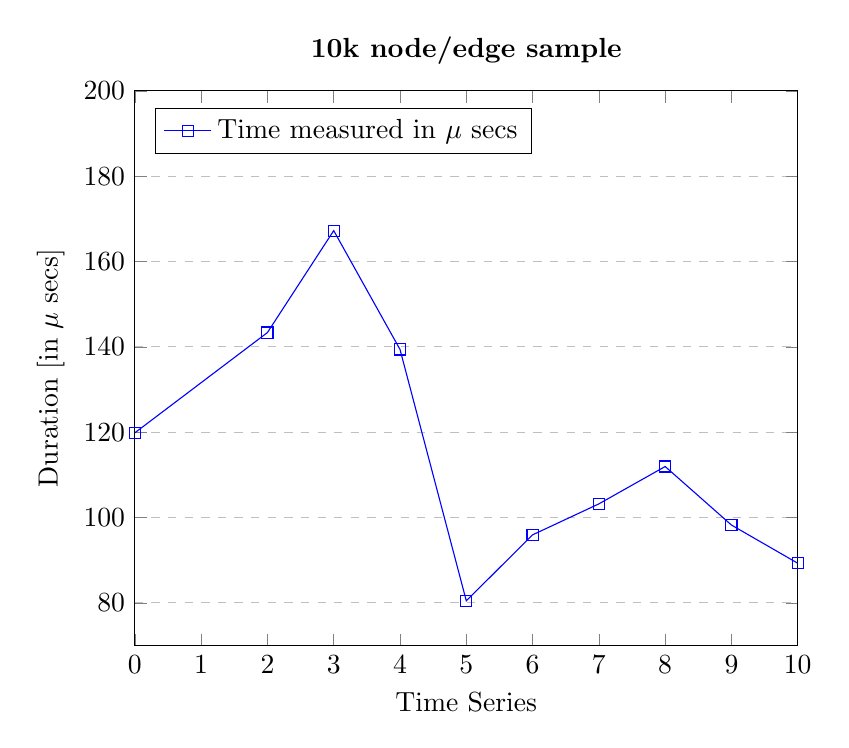
\begin{tikzpicture}

\begin{axis}[
    title=\textbf{10k node/edge sample},
    xlabel={Time Series},
    ylabel={Duration [in $\mu$ secs]},
    xmin=0, xmax=10,
    ymin=70, ymax=200,
    xtick={0,1,2,3,4,5,6,7,8,9,10},
    ytick={80,100,120,140,160,180,200},
    legend pos=north west,
    ymajorgrids=true,
    grid style=dashed,
]

\addplot[
    color=blue,
    mark=square,
    ]
    coordinates {
    (0,119.87)(2,143.37)(3,167.26)(4,139.41)(5,80.49)(6,95.95)(7,103.21)(8,111.97)(9,98.25)(10,89.30)
    };
    \legend{Time measured in $\mu$ secs}
    
\end{axis}
\end{tikzpicture}\newline\newline


%==================SEPARATOR========================%


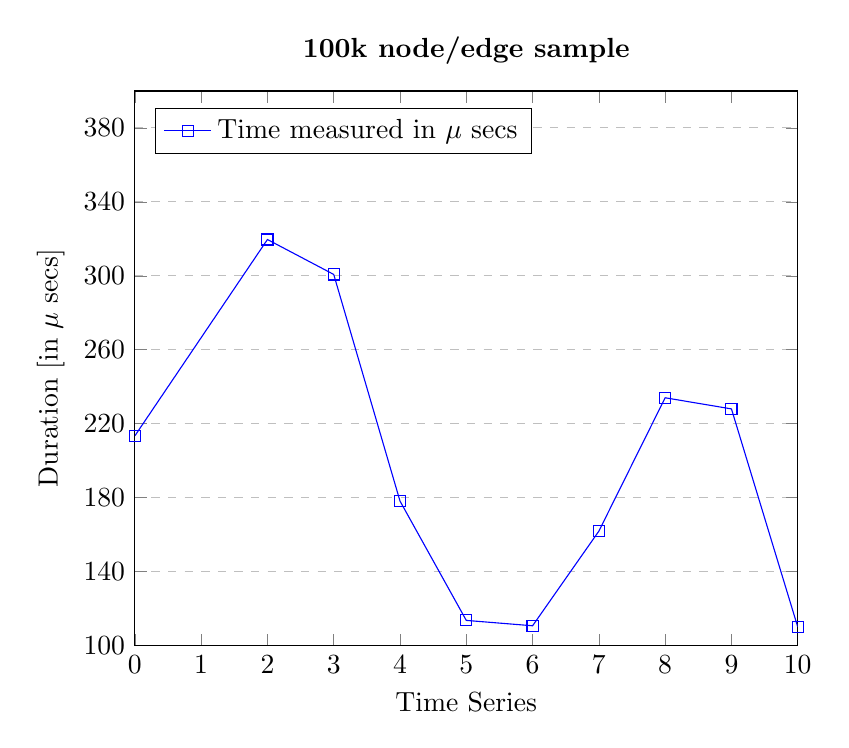
\begin{tikzpicture}

\begin{axis}[
    title=\textbf{100k node/edge sample},
    xlabel={Time Series},
    ylabel={Duration [in $\mu$ secs]},
    xmin=0, xmax=10,
    ymin=100, ymax=400,
    xtick={0,1,2,3,4,5,6,7,8,9,10},
    ytick={100,140,180,220,260,300,340,380},
    legend pos=north west,
    ymajorgrids=true,
    grid style=dashed,
]

\addplot[
    color=blue,
    mark=square,
    ]
    coordinates {
    (0,213.45)(2,319.64)(3,300.75)(4,178.15)(5,113.60)(6,110.70)(7,161.90)(8,234.03)(9,228.01)(10,110.09)
    };
    \legend{Time measured in $\mu$ secs}
    
\end{axis}
\end{tikzpicture}\newline\newline

%==================SEPARATOR========================%


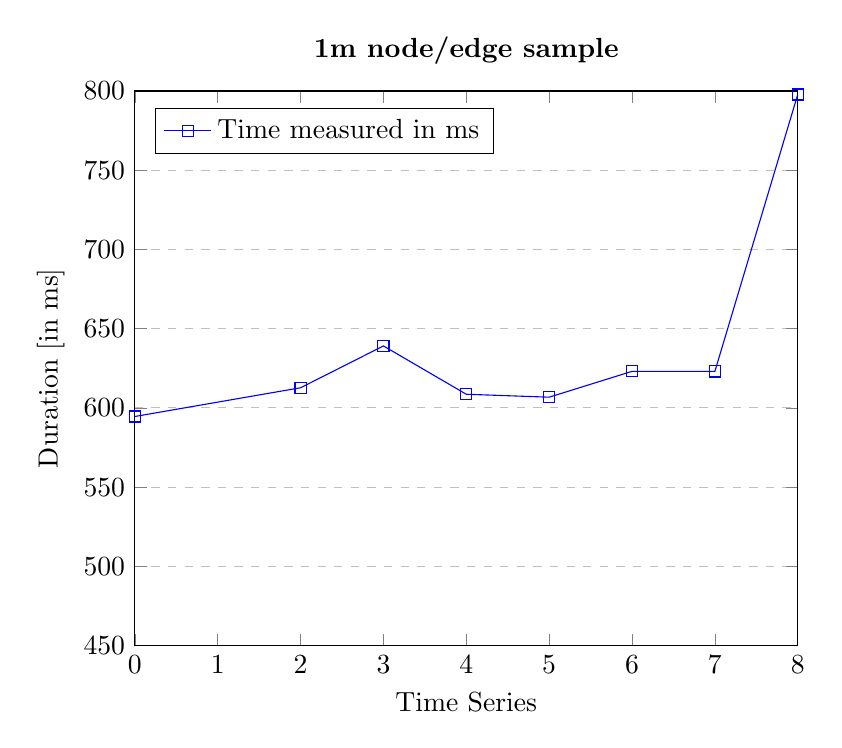
\begin{tikzpicture}

\begin{axis}[
    title=\textbf{1m node/edge sample},
    xlabel={Time Series},
    ylabel={Duration [in ms]},
    xmin=0, xmax=8,
    ymin=450, ymax=800,
    xtick={0,1,2,3,4,5,6,7,8},
    ytick={450,500,550,600,650,700,750,800},
    legend pos=north west,
    ymajorgrids=true,
    grid style=dashed,
]

\addplot[
    color=blue,
    mark=square,
    ]
    coordinates {
    (0,594.56)(2,612.69)(3,639.08)(4,608.59)(5,606.74)(6,623.04)(7,623.00)(8,797.76)
    };
    \legend{Time measured in ms}
    
\end{axis}
\end{tikzpicture}\newline\newline

\end{document}